\chapter{Computational QFT}

\begin{frame}
There are several tools which allows for the generation of models of particle physics models like LanHEP \cite{Semenov:2008jy} 
\begin{center}
  \url{http://theory.sinp.msu.ru/~semenov/lanhep.html},
\end{center}
or FeynRules \cite{Christensen:2008py}
\begin{center}
  \url{http://feynrules.phys.ucl.ac.be/}\,.
\end{center}

This kind of programs are able to generate the output required for other programs which make the calculation of Feynman diagrams and integration over multi-particle phase space. CalcHEP:
\begin{center}
  \url{http://theory.sinp.msu.ru/~pukhov/calchep.html}
\end{center}
for example, is able to calculate cross section and decays widths at tree level.

\end{frame}

In this chapter we will illustrate the use LanHEP+CalcHEP

\section{LanHEP}

\begin{frame}[fragile,allowframebreaks]{}
After download the source code from the \url{http://theory.sinp.msu.ru/~pukhov/calchep.html} to some \lstinline{DIR}, 
\begin{itemize}
\item Note that the \lstinline{tar.gz} file name depends on the current version. At the moment of this writing this was \lstinline{lhep311.tar.gz}. To directly download this file use:
\begin{lstlisting}
$ wget http://theory.sinp.msu.ru/~semenov/lhep311.tar.gz
\end{lstlisting}
where \lstinline{\$} is to indicate that the command is to be written in the shell of your Linux session\footnote{An introduction to scientific computing is at \url{http://gfif.udea.edu.co/cf} }.
To uncompress the file:\\
\begin{lstlisting}
  $ tar -zxvf DIR/lhep311.tar.gz
\end{lstlisting}

\item Go to the created directory
\begin{lstlisting}
  $ cd lanhep311
\end{lstlisting}

\item To compile and create the executable of the program (\lstinline{lhep}):\\
\begin{lstlisting}
$ make
\end{lstlisting}
\end{itemize}


The input of LanHEP are files were the Lagrangian of some model is written in a symbolic way. Then, the LanHEP executable process the input files and generates four outputfiles which are the input for the CalcHEP program. For example, in the LanHEP dir

\begin{lstlisting}
$ ./lhep stand.mdl
\end{lstlisting}
Here \lstinline{./lhep} command, search for the file in the defaul directory \lstinline{mdl/stand.mdl}. If there are no erros printed, for files are created:
\begin{lstlisting}
 ls *4.mdl
 func4.mdl  lgrng4.mdl  prtcls4.mdl  vars4.mdl
\end{lstlisting}
\end{frame}
%%%%%%%%

\section{CalcHEP}
\begin{frame}[fragile,allowframebreaks]{}
The installation of CalcHEP is similar. In Ubuntu you must be sure to have \lstinline{libx11-dev} package, in addion to the C and Fortran compilers:
\begin{lstlisting}
$ sudo apt-get install libx11-dev build-essential gfortran
\end{lstlisting}
In the CalcHEP directory:
\begin{lstlisting}
$ make
\end{lstlisting}

To use CalcHEP you must first create a directory with the required files. This is achieved with the CalcHEP command
\begin{lstlisting}
$ ./mkUsrDir YourModel
\end{lstlisting}
A directory \lstinline{YourModel} is created with several files and directories inside. By default, a \lstinline{models} directory is created with two set of \lstinline{.mdl} files, corresponding to two versions of the Standard Model:
\begin{lstlisting}
$ ls YourModel/models/
func1.mdl  lgrng1.mdl  prtcls1.mdl   vars1.mdl  
func2.mdl  lgrng2.mdl  prtcls2.mdl   vars2.mdl
\end{lstlisting}

From the \lstinline{YourModel} directory in CalcHEP, run the command
\begin{lstlisting}
./calchep
\end{lstlisting}
A new window must appear with the info of CalcHEP and the loaded models in \lstinline{YourModel/models}. To navigate through this window, use the arrows keys and the \lstinline{<ESC>} key to navigate back into the menus.  
\end{frame}

\section{LanHEP/CalcHEP}

\begin{frame}[fragile,allowframebreaks]{}
The sample \lstinline{.mdl} files in the \lstinline{mdl} directory of LanHEP must be modified in order to generate the proper CalcHEP input files. From the LanHEP directory
\begin{lstlisting}
$ mkdir sm
$ cd sm
$ wget --no-check-certificate \
   https://github.com/rescolo/LanHEP/raw/release/sm/sm.mdl
$ wget --no-check-certificate \
   https://github.com/rescolo/LanHEP/raw/release/sm/sm_tex.mdl

$ ../lhep sm.mdl
\end{lstlisting}
The four CalcHEP input files:
\begin{lstlisting}
func1.mdl  lgrng1.mdl  prtcls1.mdl   vars1.mdl  
\end{lstlisting}
are then created.

From CalcHEP directoty:
\begin{lstlisting}
$ ./mkUsrDir sm
$ cd sm/models
$ rm * 
\end{lstlisting}
then copy the \lstinline{*1.mdl} files to the \lstinline{sm/models}, and from the \lstinline{sm} CalcHEP directory run \lstinline{./calchep}.

In order to understand the structure of the LanHEP files consider the following skeleton:
\begin{lstlisting}[numbers=left,xleftmargin=1cm,numberstyle=\tiny,escapeinside={(*}{*)}]
model 'MODEL NAME'/N.
% The coments are either this way
/* or this other way */

use file_tex.

prtcprop pdg.

prtcformat fullname:'  Full Name  ',
           name:' P ',
           aname:' aP ',
           pdg:' number ',
           spin2, mass, width, color, aux,
           texname:'>  LaTeX P name  <',
           atexname:'>  LaTeX aP name < '.

parameter  VAR  = VALUE : 'Description'.

particle_type  
	particle/Antiparticle: ('name', property name=VALUE, ...).

lterm  	Write here the Lagrangian in a LaTeX--like format

prtcprop pdg:(Particle=PDF code,...).

SetEM(A,EE). %check charge conservation
CheckHerm.
\end{lstlisting}
In line 1, \lstinline{N} is an integer that will identify the four output files. The file in line 5 will contain the \LaTeX{} definitions of the used particles. In lines 7-15, the format of the table \lstinline{prtclN.mdl}, as required by CalcHEP, is defined: A new column with the PDG number for the particle.  In line 17, the general form to declarate a variable is established, while the lines 19-20 are the generic declaration for a particle. The final commands in 26 and 27 is to check the consistency of the defined model. 
As a simple illustration consider the simple case of QED:
\begin{lstlisting}
model 'QED: e, mu tau'/1.

use qed3g_tex.

prtcprop pdg.

%prtc1.mdl is one of the output files of LanHEP. To make
% it compatible with CalcHEP we need to change their format
% to include the PDG particle number in the third column
 
prtcformat fullname:'  Full Name  ',
           name:' P ',
           aname:' aP ',
           pdg:' number ',
           spin2, mass, width, color, aux,
           texname:'>  LaTeX P name  <',
           atexname:'>  LaTeX aP name < '.

parameter  EE  = 0.31333 : 'Electromagnetic coupling constant (<->1/128)'.

vector  
	A/A: (photon, gauge).

spinor 		e1:(electron),
		e2:(muon, mass Mm  = 0.1057),
		e3:('tau-lepton', mass Mt  = 1.777).

% fermion interaction with gauge fields

lterm  	anti(psi)*gamma*(i*deriv - EE*A)*psi
		where 
			psi=e1;
			psi=e2;
			psi=e3.

% gauge bosons Lagrangian

lterm -F**2/4   where 
	F=deriv^mu*A^nu-deriv^nu*A^mu.

%set PDG particle numbers:

prtcprop pdg:(A=22,e1=11, e2=13, e3=15).

SetEM(A,EE). %check charge conservation
CheckHerm.
\end{lstlisting}
where the required file \lstinline{qed3g_tex.mdl} is
\begin{lstlisting}
SetTexName([e1=e,E1='\\bar{e}']).
SetTexName([e=e,E='\\bar{e}']).
SetTexName(['e1.c'='e^c','E1.c'='\\bar{e}^c']).
SetTexName(['e.c'='e^c','E.c'='\\bar{e}^c']).
SetTexName([e2='\\mu',E2='\\bar{\\mu}']).
SetTexName([e3='\\tau',E3='\\bar{\\tau}']).
SetTexName([m='\\mu',M='\\bar{\\mu}']).
SetTexName([l='\\tau',L='\\bar{\\tau}']).

SetTexName([EE=e]).

SetTexName([Me='M_e', Mm='M_\\mu', Mt='M_\\tau']).
\end{lstlisting}

Running with the option \lstinline{-tex}:
\begin{lstlisting}
../lhep qed3g.mdl
\end{lstlisting}
the following output is generated
\begin{itemize}
\item \lstinline{lgrng1.tex}
\begin{center}

\begin{tabular}{|l|l|} \hline
Fields in the vertex & Variational derivative of Lagrangian by fields \\ \hline
$\bar{e}{}_{a }$ \phantom{-} $e{}_{b }$ \phantom{-} ${A}_{\mu }$ \phantom{-}  &
        $- e\cdot \gamma_{a b}^\mu $\\[2mm]
$\bar{\mu}{}_{a }$ \phantom{-} $\mu{}_{b }$ \phantom{-} ${A}_{\mu }$ \phantom{-}  &
        $- e\cdot \gamma_{a b}^\mu $\\[2mm]
$\bar{\tau}{}_{a }$ \phantom{-} $\tau{}_{b }$ \phantom{-} ${A}_{\mu }$ \phantom{-}  &
        $- e\cdot \gamma_{a b}^\mu $\\ \hline
\end{tabular}

\end{center}



\item \lstinline{prtcls1.tex}:
  \begin{center}
    \begin{tabular}{|cc|l|c|c|c|l|} \hline
P & aP & Name & Spin  & EM charge & Color & Comment \\ \hline
$A_{\mu }$&$A_{\mu }$&photon        &1           & $\phantom{-}0$ &1    &gauge\\
$e{}_{a}$ &$\bar{e}{}_{a}$&electron      &$1/2$       &$\phantom{-}1$ &1    &   \\
$\mu{}_{a}$&$\bar{\mu}{}_{a}$&muon          &$1/2$       &$\phantom{-}1$ &1    &   \\
$\tau{}_{a}$&$\bar{\tau}{}_{a}$&tau-lepton    &$1/2$       &$\phantom{-}1$ &1    &   \\ \hline
\end{tabular}
  \end{center}

\item \lstinline{vars1.tex}
  \begin{center}
    \begin{tabular}{|l|l|l|} \hline
Parameter & Value & Comment \\ \hline
EE    &0.31333             &Electromagnetic coupling constant (1/128) \\
Mm    &0.1057              &mass of muon \\
Mt    &1.777               &mass of tau-lepton \\ \hline
\end{tabular}
  \end{center}
\end{itemize}

With the command
\begin{lstlisting}
$ ../lhep qed3g.mdl
\end{lstlisting}
the same files are generated by in the format of CalcHEP.

parameter is for constants to be exported to tables, while let is only for internal LanHEP variables.

In CalcHEP
\begin{lstlisting}
\$ ./mkUsrDir qed3g
\$ cd qed3g/models
\$ rm *
#copy the files: func1.mdl, lgrng1.mdl prtcls1.mdl, vars1.mdl here
\$ cd ..
\$ ./calchep
\end{lstlisting}
The window in Fig.~\ref{fig:calchep1}
\begin{figure}
  \centering
  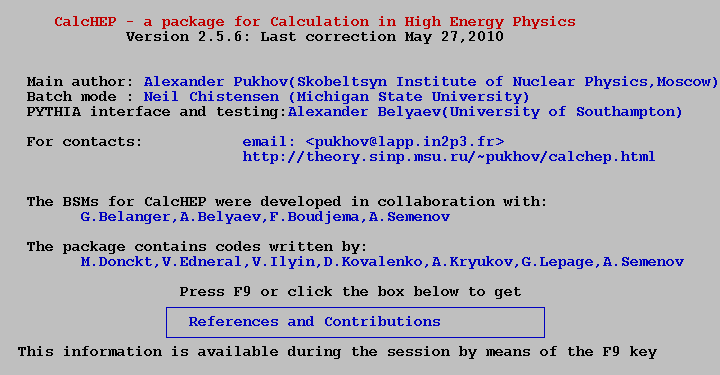
\includegraphics[scale=0.45]{calchep1}
  \caption{CalcHEP welcome window}
  \label{fig:calchep1}
\end{figure}
After hit \lstinline{<Enter>}, the window with the model should appears as shown in Fig.~\ref{fig:calchep2}
\begin{figure}
  \centering
  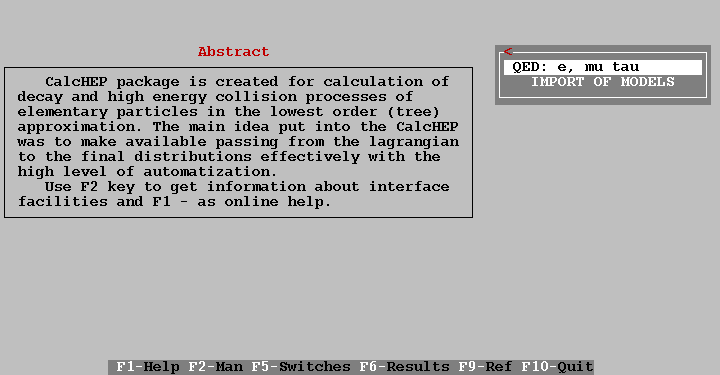
\includegraphics[scale=0.45]{calchep2}
  \caption{CalcHEP model window}
  \label{fig:calchep2}
\end{figure}
To test that the model was loaded without errors:
\begin{lstlisting}
QED: e, mu tau -> Edit Model -> Check Model
\end{lstlisting}
A message with \lstinline{The model is OK}, should popup.

After returning to the model window in Fig.~\ref{fig:calchep2}, we could calculate some process:
\begin{lstlisting}
QED: e, mu tau -> Enter Process 
\end{lstlisting}
and enter the process \lstinline{e1,E1 -> e2,E2} ($e^+ e^-\to \mu^+\mu^-$) as shown in the Fig:~\ref{fig:calchep3}
\begin{figure}
  \centering
  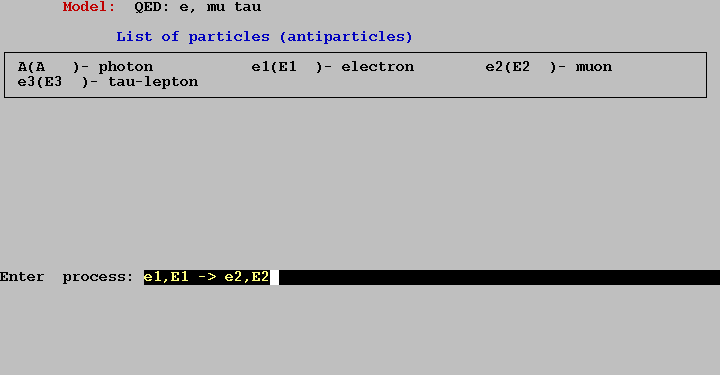
\includegraphics[scale=0.45]{calchep3}
  \caption{CalcHEP process window}
  \label{fig:calchep3}
\end{figure}
After \lstinline{<Enter>}, the window to calculate the process should appears, as in Fig.~\ref{fig:calchep4}
\begin{figure}
  \centering
  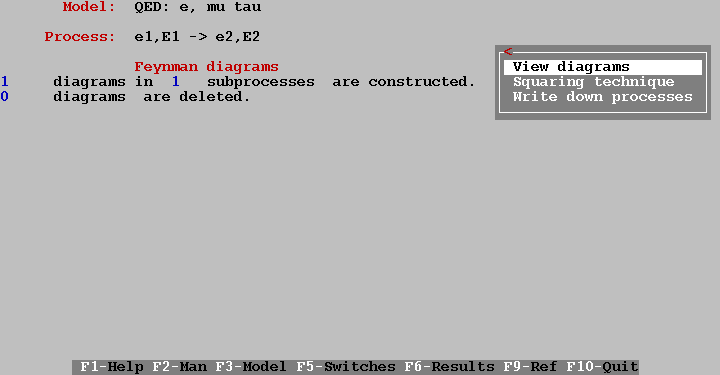
\includegraphics[scale=0.45]{calchep4}
  \caption{CalcHEP calculation window}
  \label{fig:calchep4}
\end{figure}
In addition to \lstinline{View diagrams}, we can calculate the process with the sequence
\begin{lstlisting}
Squaring technique -> Symbolic calculations -> C-compiler
\end{lstlisting}
Then a new window with the process details should appears, as displayed in Fig.~\ref{fig:calchep5}
\begin{figure}
  \centering
  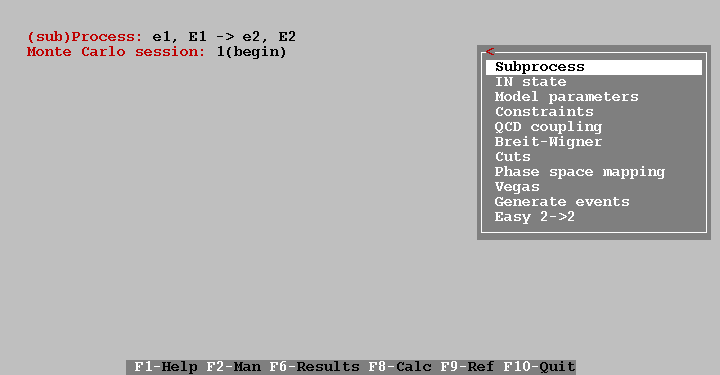
\includegraphics[scale=0.45]{calchep5}
  \caption{CalcHEP calculation window}
  \label{fig:calchep5}
\end{figure}
After adjust the input parameters at your convenience, we could just calculate the process with, in this case: \lstinline{Easy 2-2}, to obtain the result displayed in ~\ref{fig:calchep6}
\begin{figure}
  \centering
  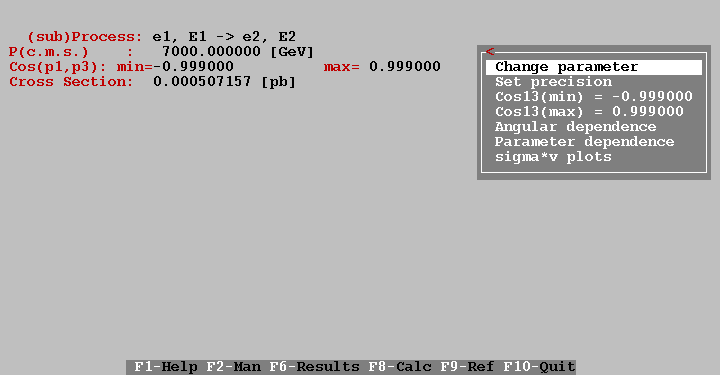
\includegraphics[scale=0.45]{calchep6}
  \caption{CalcHEP results window}
  \label{fig:calchep6}
\end{figure}
e.g, for center of mass energy of 14 TeV (7 TeV per beam) we could have:
\begin{align}
  \sigma(e^+\,e^-\to \mu^+\mu^-)=5\times 10^{-4}\,\text{pb}\,
\end{align}
\begin{itemize}
\item \textbf{Exercise}:
Repeat the previous calculation, but for one center of mass energy of 200 GeV.
\end{itemize}

For the Standard Model the Yukawa Lagrangian that couple the down fermions with the boson scalar is written in the interaction basis:
\begin{equation}\label{eq:base_in}
  \mathcal{-L}_Y\sim\overline{D'}M_D P_R D'H + {\rm h.c}\; ,
\end{equation}
with $D'=V^{\dagger}D$, we can write the eq. (\ref{eq:base_in}) in the mass eigenstates 
as
\begin{align}
  \mathcal{-L}_Y\sim\overline{D}M_D^{dia}P_RDH + {\rm h.c}
\end{align} 
where
\begin{equation}\label{eq:masa_matrix}
  M_D^{dia}=VM_DV^{\dagger}
\end{equation}
 Investing the equation \ref{eq:masa_matrix} and replacing in \eqref{eq:base_in}  we can write in the interaction eigenstates:
 \begin{align}
   \mathcal{-L}_Y\sim (\overline{D'}V^{\dagger})(M_D^{dia}V)P_R D'H + {\rm h.c}
 \end{align}
Expanding we get
. . .
which is just the expresion in the Standard Model file  



\end{frame}

%%% Local Variables: 
%%% mode: latex
%%% TeX-master: "beyond.beamer.tex"
%%% End: